\documentclass{article}
\usepackage{graphicx}
\usepackage{amsmath}

\author{Fraser Paterson 22258324}
\title{MATH3024 Project}

\begin{document}

\maketitle

\section*{Introduction}

This is the project for Fraser Paterson

\section*{Questions}

\subsection*{Question 1}

The system for question 1 is as follows:

$$\dot{x} = \alpha(y - x - f(x))$$
$$\dot{y} = x - y + z$$
$$\dot{x} = -\beta y$$
where
$$f(x) = bx + \frac{1}{2}(a - b)[|x + 1| - |x - 1|]$$
and $\alpha = 10.0, \beta = 14.87, a = -1.27, b = -0.68$

\paragraph{1.a} This is as described in my interem report.

\paragraph{1.b} For an x to x coupling we take a copy of the entire system and add the
difference in the x coordinates, multiplied by the coupling strength: $\sigma$, to both x coordinates
in each respective system. Let each coordinate dynamics
be given by a primed value, hence we have:

$$\dot{x} = \alpha(y - x - f(x)) + \sigma(x' - x)$$
$$\dot{y} = x - y + z\newline$$
$$\dot{x} = -\beta y\newline$$
$$\dot{x'} = \alpha(y' - x' - f(x')) +\sigma(x - x')$$
$$\dot{y'} = x' - y' + z'$$
$$\dot{x'} = -\beta y'$$
where
$$f(x') = bx + \frac{1}{2}(a - b)[|x' + 1| - |x' - 1|]$$
and the parameters remain as above.

To analyse the stability of the coupling for any given $\sigma \in [0, 10.0]$ we define the following
errors in each respective component of the coupled dynamics:

$$e_{x} = x - x'$$
$$e_{y} = y - y'$$
$$e_{z} = z - z'$$

Substituting in each respective expression for x and x' into these error equations, we have:

$$e_{x} = \alpha(e_{y} - e_{x} - (f(x) - f(x'))) - 2\sigma e_{x}$$


Note, that by the intermidiate value theorem $f(x) - f(x') = f'(\eta)(x - x')$ we may express the above as:

$$e_{x} = \alpha(e_{y} - e_{x} - f'(\eta)e_{x}) - 2\sigma e_{x}$$

Now, $f'(\eta)$ = a or b. Hence let $f'(\eta) = \xi$ and so
we have: $e_{x} = (-\alpha - \alpha\xi - 2\sigma)e_{x} + \alpha e_{y}$. Performing a
similar set of substitutions for the y and z errors yields the full error dynamics:

$$e_{x} = (-\alpha - \alpha\xi - 2\sigma)e_{x} + \alpha e_{y}$$
$$e_{y} = e_{x} - e_{y} + e_{z}$$
$$e_{z} = -\beta e_{y}$$

Expressing the error dynamics as a matrix equation:


$$
\begin{pmatrix}
    \dot{e_{x}} \\
    \dot{e_{y}} \\
    \dot{e_{z}} \\
\end{pmatrix} =
\begin{pmatrix}
-\alpha - \alpha\xi - 2\sigma & \alpha & 0\\
1 & -1 & 0\\
0 & -\beta & 0
\end{pmatrix}
\begin{pmatrix}
    e_{x} \\
    e_{y} \\
    e_{z} \\
\end{pmatrix}
$$


If we are to have stable synchronisation, we require $\sigma$ such that all the eigenvalues of
the above matrix are real and negative, thus we find the roots of the corresponding characteristic
polynomial:

$$\lambda^3 + (\alpha + \alpha\xi + 2\sigma + 1)\lambda^2 + (\alpha\xi + 2\sigma + \beta)\lambda + (\alpha\beta + \alpha\xi\beta + 2\sigma\beta) = 0$$

Now for any polynomial of the form:

$$\lambda^3 + a_{2}\lambda^2 + a_{1}\lambda + a_{0} = 0$$


The Routh-Hurwitz criterion specifies the following 2 conditions on the coefficents,
sufficent to gurantee that all roots are real and negative. These are:

$$a_{0} > 0, a_{1} > 0 ~~ and ~~ a_{2}a_{1} - a_{0} > 0$$


\subsection*{Question 2}
The maths for question 2
The following is a graph:

\begin{figure}[h]
\centering
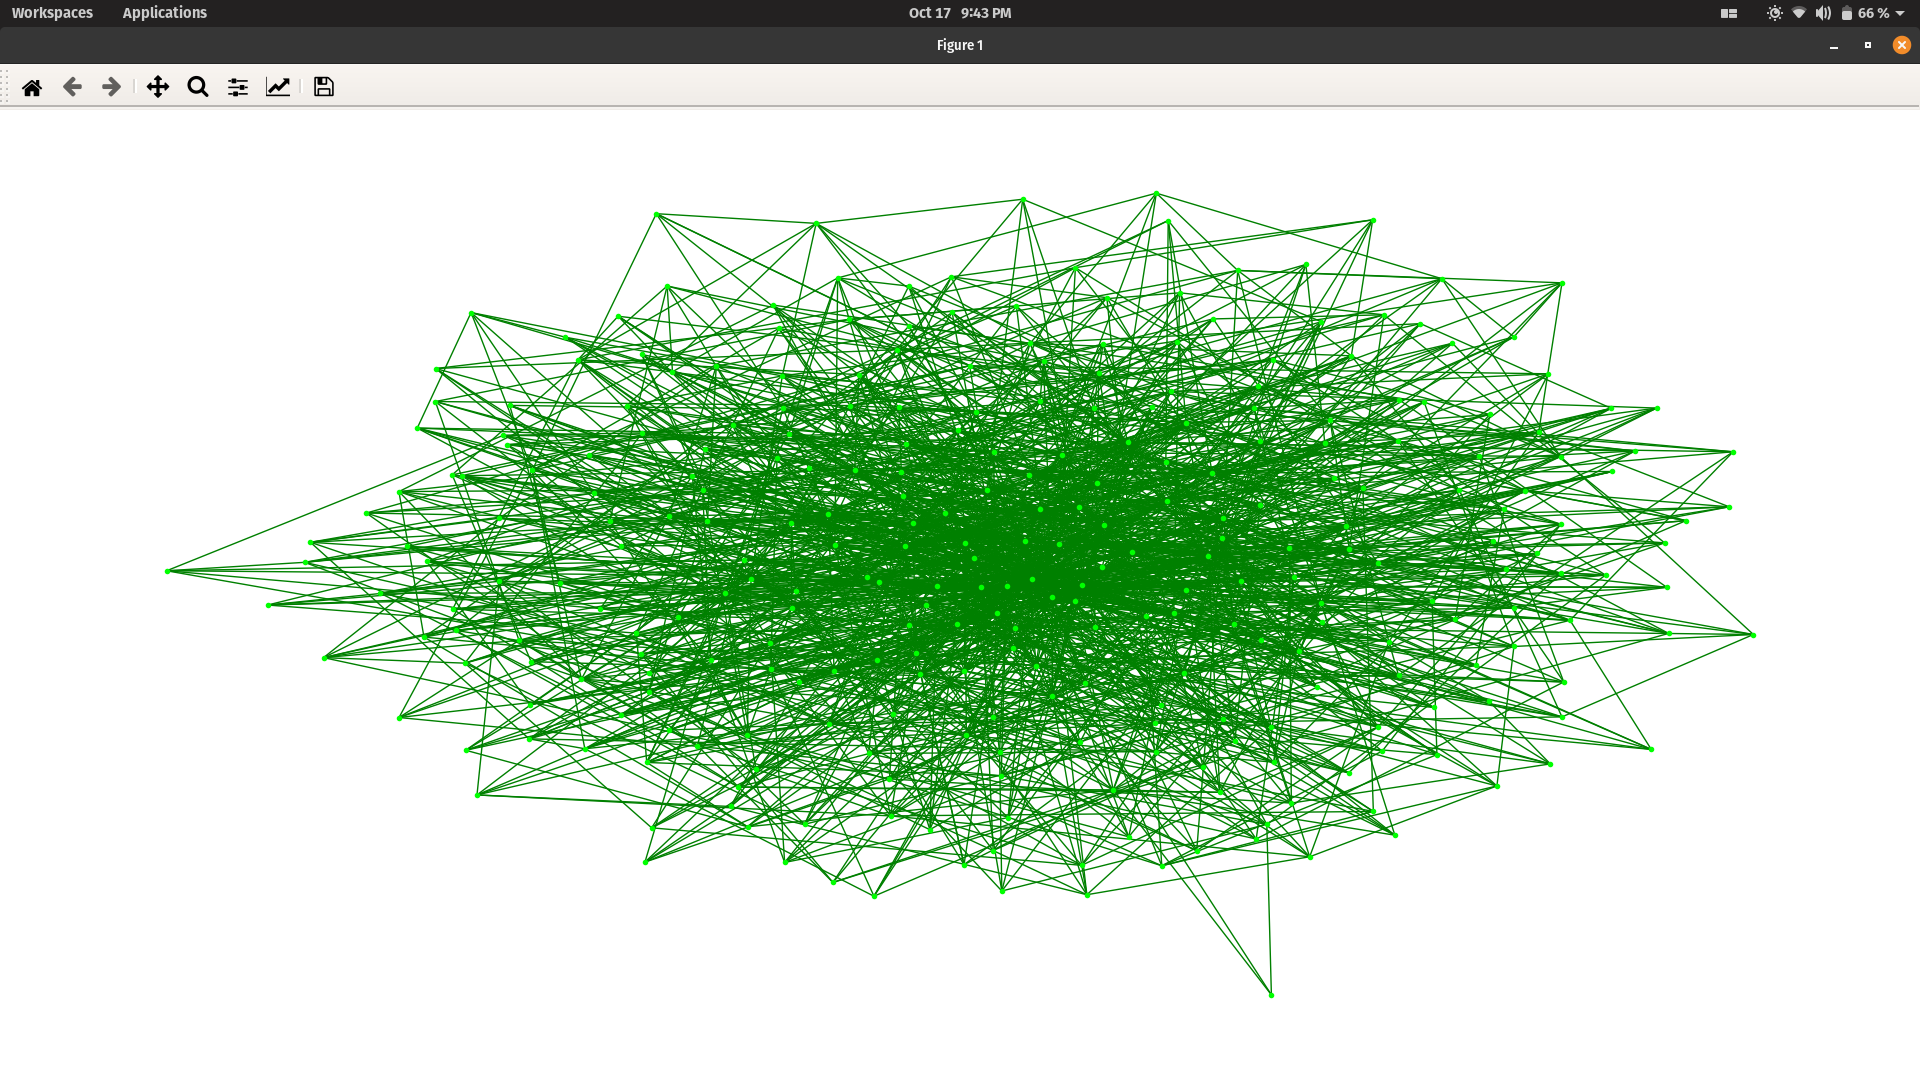
\includegraphics[width = 4in]{Screenshot from 2021-10-17 21-43-29.png}
\caption{A random graph with 300 vertices}
\end{figure}


\subsection*{Question 3}
Maths for question 3


\end{document}
